\chapter{ Adaptive Control}

An adaptive controller uses some adaption rule to change the parameters of the controller, with the target the drive the error of the system to zero. In this approach the dynamic equation of the robot will the separated into a know part  $\mathbf{Y}(.)$ and a part, which have to be adapted $\varphi$. In this case the masses of the system are assumed to be unknown. 
The following equation the known part can be calculated:
\begin{equation*}
\mathbf{Y}(.)\varphi = \mathbf{M}(\ddot{\mathbf{q}}_D + \Lambda \dot{\mathbf{e}}) + \mathbf{V}_m(\dot{\mathbf{q}}_D + \Lambda \mathbf{e})+ \mathbf{g}
\end{equation*}

Since the masses are unknown the parameter vector $\varphi$ consists of two masses and the rest of the dynamic equations is put into  $\mathbf{Y}(.)$, which leads to:
\begin{align*}
Y_{11} =& \left(\ddot{q}_{D,1} - \lambda_1 \left(\dot{q}_{1} - \dot{q}_{D,1}\right)\right) {a_1}^2 + g \cos\!\left(q_1\right) a_1\\
Y_{12} =& g \left(a_2 \cos\!\left(q_1 + q_2\right) + a_1 \cos\!\left(q_1\right)\right) + \left(\ddot{q}_{D,1} - \lambda_1 \left(\dot{q}_{1} - \dot{q}_{D,1}\right)\right) \left({a_1}^2 + 2 \cos\!\left(q_2\right) a_1 a_2 + {a_2}^2\right)\\& + a_2 \left(\ddot{q}_{D,2} - \lambda_2 \left(\dot{q}_{2} - \dot{q}_{D,2}\right)\right) \left(a_2 + a_1 \cos\!\left(q_2\right)\right) - 2 a_1 a_2 \dot{q}_{2} \sin\!\left(q_2\right) \left(\dot{q}_{D,1} - \lambda_1 \left(q_1 - q_{D,1}\right)\right)\\& - a_1 a_2 \dot{q}_{2} \sin\!\left(q_2\right) \left(\dot{q}_{D,2} - \lambda_2 \left(q_2 - q_{D,2}\right)\right)\\
Y_{21} =&                    0\\
Y_{22} =& {a_2}^2 \left(\ddot{q}_{D,2} - \lambda_2 \left(\dot{q}_{2} - \dot{q}_{D,2}\right)\right) + a_2 \left(\ddot{q}_{D,1} - \lambda_1 \left(\dot{q}_{1} - \dot{q}_{D,1}\right)\right) \left(a_2 + a_1 \cos\!\left(q_2\right)\right) + a_2 g \cos\!\left(q_1 + q_2\right)\\& + a_1 a_2 \dot{q}_{1} \sin\!\left(q_2\right) \left(\dot{q}_{D,1} - \lambda_1 \left(q_1 - q_{D,1}\right)\right)
\end{align*}
Additional a function for the tracking error is needed:
\begin{equation*}
\mathbf{r} = \Lambda \mathbf{e} + \dot{\mathbf{e}}
\end{equation*}
$\Lambda$ is again a diagonal matrix which is positive definite. With these components, the control law can be built:
\begin{gather*}
\tau_c = \mathbf{Y}(.)\hat{\varphi} + \mathbf{K}_v \mathbf{r}
\intertext{where:}
\begin{tabular}{>{$}l<{$} @{${}:{}$} l}
\hat{\varphi} & approximated system parameters\\
\mathbf{K}_v & diagonal gain matrix, positive definite
\end{tabular}\nonumber
\end{gather*}
As a last component, the adaptation rule for the unknown parameters is needed:
\begin{gather*}
\dot{\hat{\varphi}} = \Gamma \mathbf{Y}^T(.)\mathbf{r}
\intertext{where:}
\begin{tabular}{>{$}l<{$} @{${}:{}$} l}
\Gamma & diagonal matrix which defines adaptation speed
\end{tabular}\nonumber
\end{gather*}

The simulation results in figure \ref{fig:ch6_adap1} are showing that the controller needs around 2 seconds to adapt to the right value of the masses. Caused by the initial wrong values of the  masses the torque shows a very high peak.
\begin{figure}[]
	\centering
	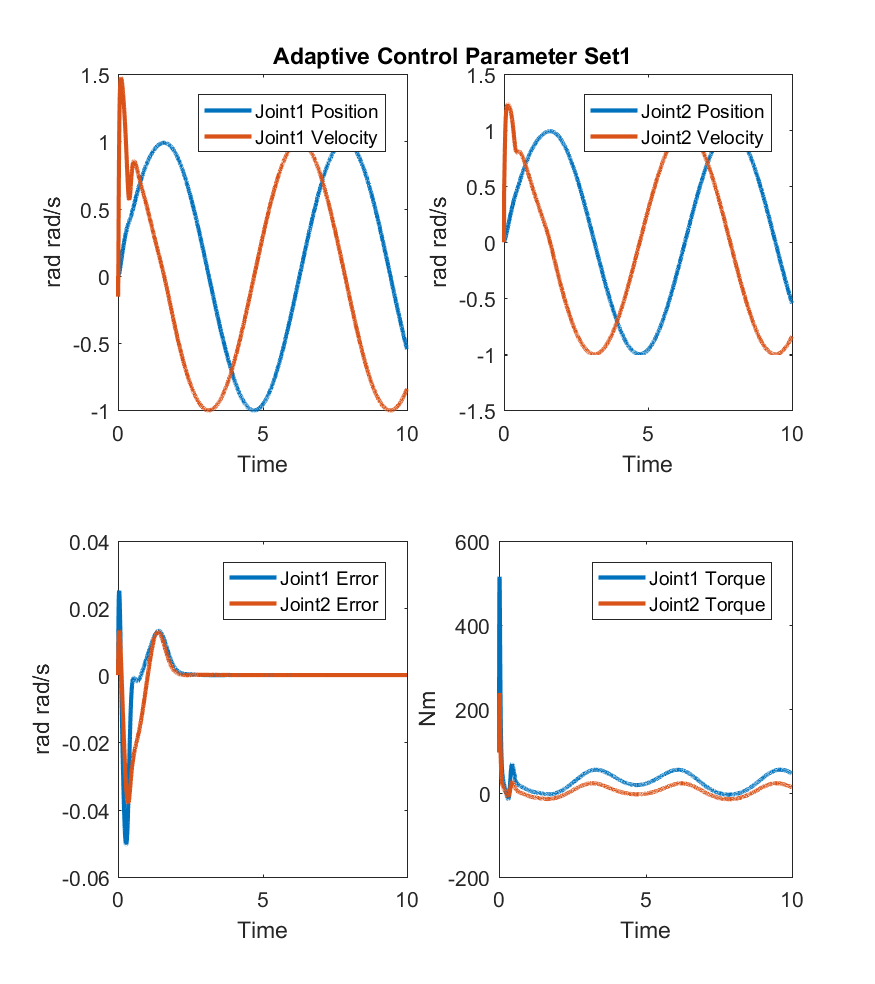
\includegraphics[width=0.85\textwidth]{pics/AdaptiveControlParameterSet1.png}\\
	\caption{Adaptive Control with $\lambda = 5, \gamma=10 $ and $k_v = 100$ }
	\label{fig:ch6_adap1}
\end{figure}

The results in figure \ref{fig:ch6_adap2} are showing that the controller needs 3 seconds to adapt. Since the controller is reacting faster the peak within the error signal is quite higher.
\begin{figure}[]
	\centering
	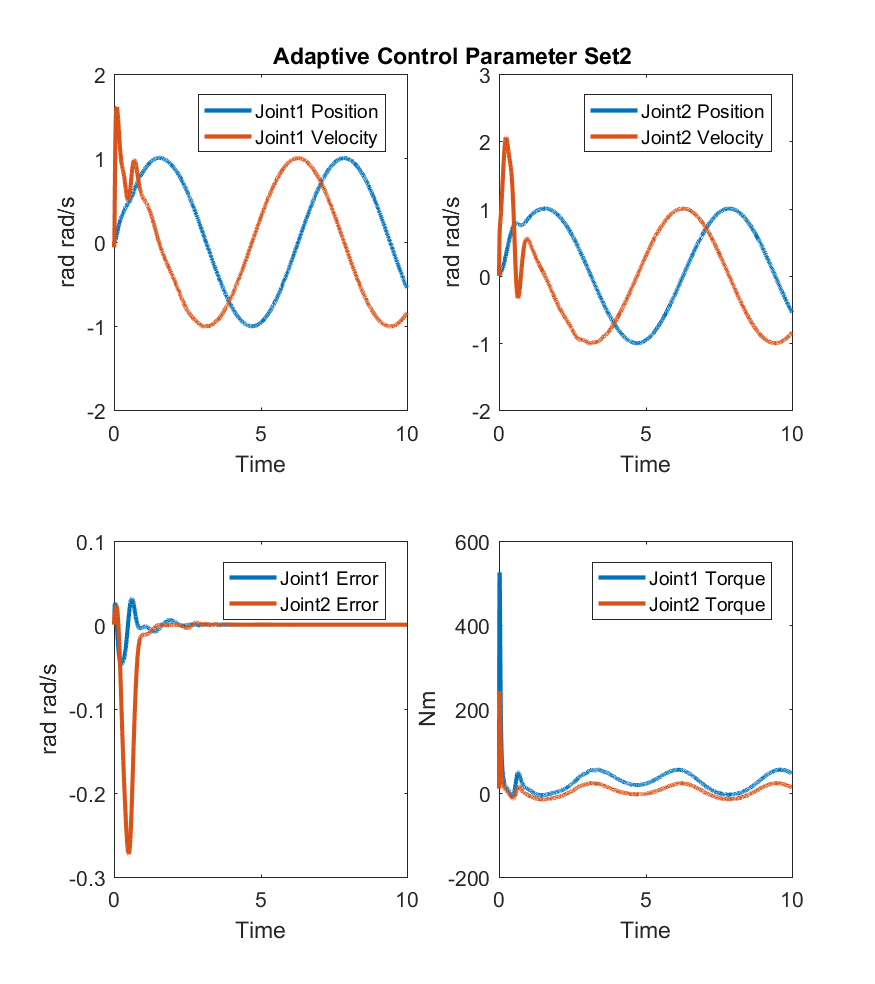
\includegraphics[width=0.85\textwidth]{pics/AdaptiveControlParameterSet2.png}\\
	\caption{Adaptive Control with $\lambda = 5, \gamma=10 $ and $k_v = 10$  }
	\label{fig:ch6_adap2}
\end{figure}

